In den vorherigen Kapiteln wurde beleuchtet, dass Agilität skaliert auf Unternehmensebene verschiedene Vorteile und  Risiken mit sich bringt und auf regelmäßige ad hoc Entscheidungen in verschiedenen Ebenen des Unternehmens angewiesen ist, um effektive Ergebnisse zu erzielen. Diese Entscheidungen sollten auf Basis von Metriken aus generalisierten Reporting-Prozessen getroffen werden, wobei diese Reporting-Prozesse, wenn möglich, automatisiert werden sollten, um Konsistenz, Regelmäßigkeit, Validität und Aktualität zu gewährleisten. Tool basierendes Reporting hat sich in vielen Unternehmen als eine erfolgreiche Automatisierungsmethode bewiesen.
Resultierend aus diesen Erkenntnissen wird an dieser Stelle ein Prozess definiert der ein Tool für einen Dokumentations- und Reporting-Prozess abbildet, aus denen anschließend ein UX-Konzept und im nächsten Kapitel eine prototypische Implementierung entwickelt werden kann.

\subsection{Prozessdefinition / Anforderungsformulierung}
Für Fortschrittsmessung und Werteorientierung müssen Zusammenhänge innerhalb eines Portfolios mit operativen Elementen, deren absoluter Fortschritt tatsächlich gemessen werden kann, dokumentiert werden können. Diese Verknüpfung muss über beliebig viele Ebenen stattfinden können, um möglichst universell und unabhängig von der Unternehmensstruktur und dem verwendeten Framework benutzbar zu sein.
Operative Elemente, hier genannt Aufgabe, haben einen veränderbaren Status an dem festgestellt werden kann, ob sie fertig sind und somit für den gemessenen Fortschritt einbezogen werden müssen. Aufgaben außerdem besitzen zudem zwei numerische Werte: Storypoints und Value. Storypoints sollen als relativer Wert die Komplexität der Umsetzung, die mit einer Aufgabe verbunden ist darstellen, während Value den Mehrwert widerspiegelt, welcher durch die Erledigung der Aufgabe entsteht. Die Bezeichnung ist in diesem Fall mit Absicht unspezifisch gewählt, um weitere Komplexität zu vermeiden und den Scope dieser Arbeit zu verkleinern, da zwischen verschiedenen Formen von Mehrwert unterschieden werden kann, wie z. B. Business-, Customer-Value oder auch interner Mehrwert. Ziel dieser Werte ist, die Aufgaben vergleichbarer zu machen, da einige Aufgaben mehr Einfluss auf den Fortschritt haben können als andere. Aufgaben im Kontext des Prototyps würden somit die Funktion der User-Stories erfüllen.

Die zuvor bereits beschriebene weitere Unterteilung in Tasks spielt für die Fortschrittsmessung oder Werteorientierung und dementsprechend auch für ein Refinement keine Rolle, da Mehrwert und Fortschritt nur entsteht, wenn eine User-Story vollständig umgesetzt wurde und wird deshalb vernachlässigt.

Damit die spezifische Struktur eines Unternehmens abgebildet werden kann, muss es möglich sein, verschiedene Ebenen anzulegen, welche die hierarchische Struktur darstellen kann, welche tatsächlich in den Unternehmen verwendet wird. Innerhalb dieser Ebenen können Elemente angelegt werden, welche mit anderen Elementen in darüber liegenden Ebenen verknüpft werden können.
Die unterste Ebene ist immer die operative Ebene, welche für gewöhnlich als Projekt bezeichnet wird. Optional können Epics verwendet werden, um Aufgaben innerhalb eines Projekts zu gruppieren, sodass mehrere Aufgaben zusammengefasst z. B. ein Feature o. ä. darstellen können.

Der Fortschritt eines Projekts resultiert aus dem Verhältnis von offenen zu erledigten Aufgaben oder Epics, wobei Storypoints und Mehrwert als Faktoren hinzugezogen werden können, um das Verhältnis zu relativieren.

Der Fortschritt eines Planungselements, welches keine Aufgabe oder Projekt ist, wird durch den Gesamtfortschritt der verknüpften Elemente aus der darunterliegenden Ebene aggregiert. Daraus ergibt sich eine Baumartige Struktur, welche die gesamte Planungsstruktur eines Unternehmens abbilden soll.

Um die Evaluierung zu erleichtern und mehrere Szenarien testbar zu machen, können mehrere dieser Strukturen innerhalb der Anwendung existieren, weshalb es eine Ebene gibt, die hier Organisation genannt wird. Organisationen können unabhängig voneinander existieren und eine vollständige Datenstruktur beinhalten.

\subsection{UX-Entwurf für die Abbildung des Prozesses}
Um den Userflow innerhalb des Prototyps darzustellen, wurde ein UX-Entwurf mit Figma entwickelt, welcher alle Funktionalitäten der Anwendung visuell abbildet und als Grundlage für das Design der Benutzeroberfläche dient. Der Entwurf ist als Klickprototyp \href{https://www.figma.com/proto/6TjaUCKvs4DjwzTDEiWxiO/Prototype?type=design&node-id=0-1&scaling=min-zoom&starting-point-node-id=2%3A61}{hier} verfügbar.

\vspace{20pt}
\begin{center}
    \begin{minipage}{\linewidth}
        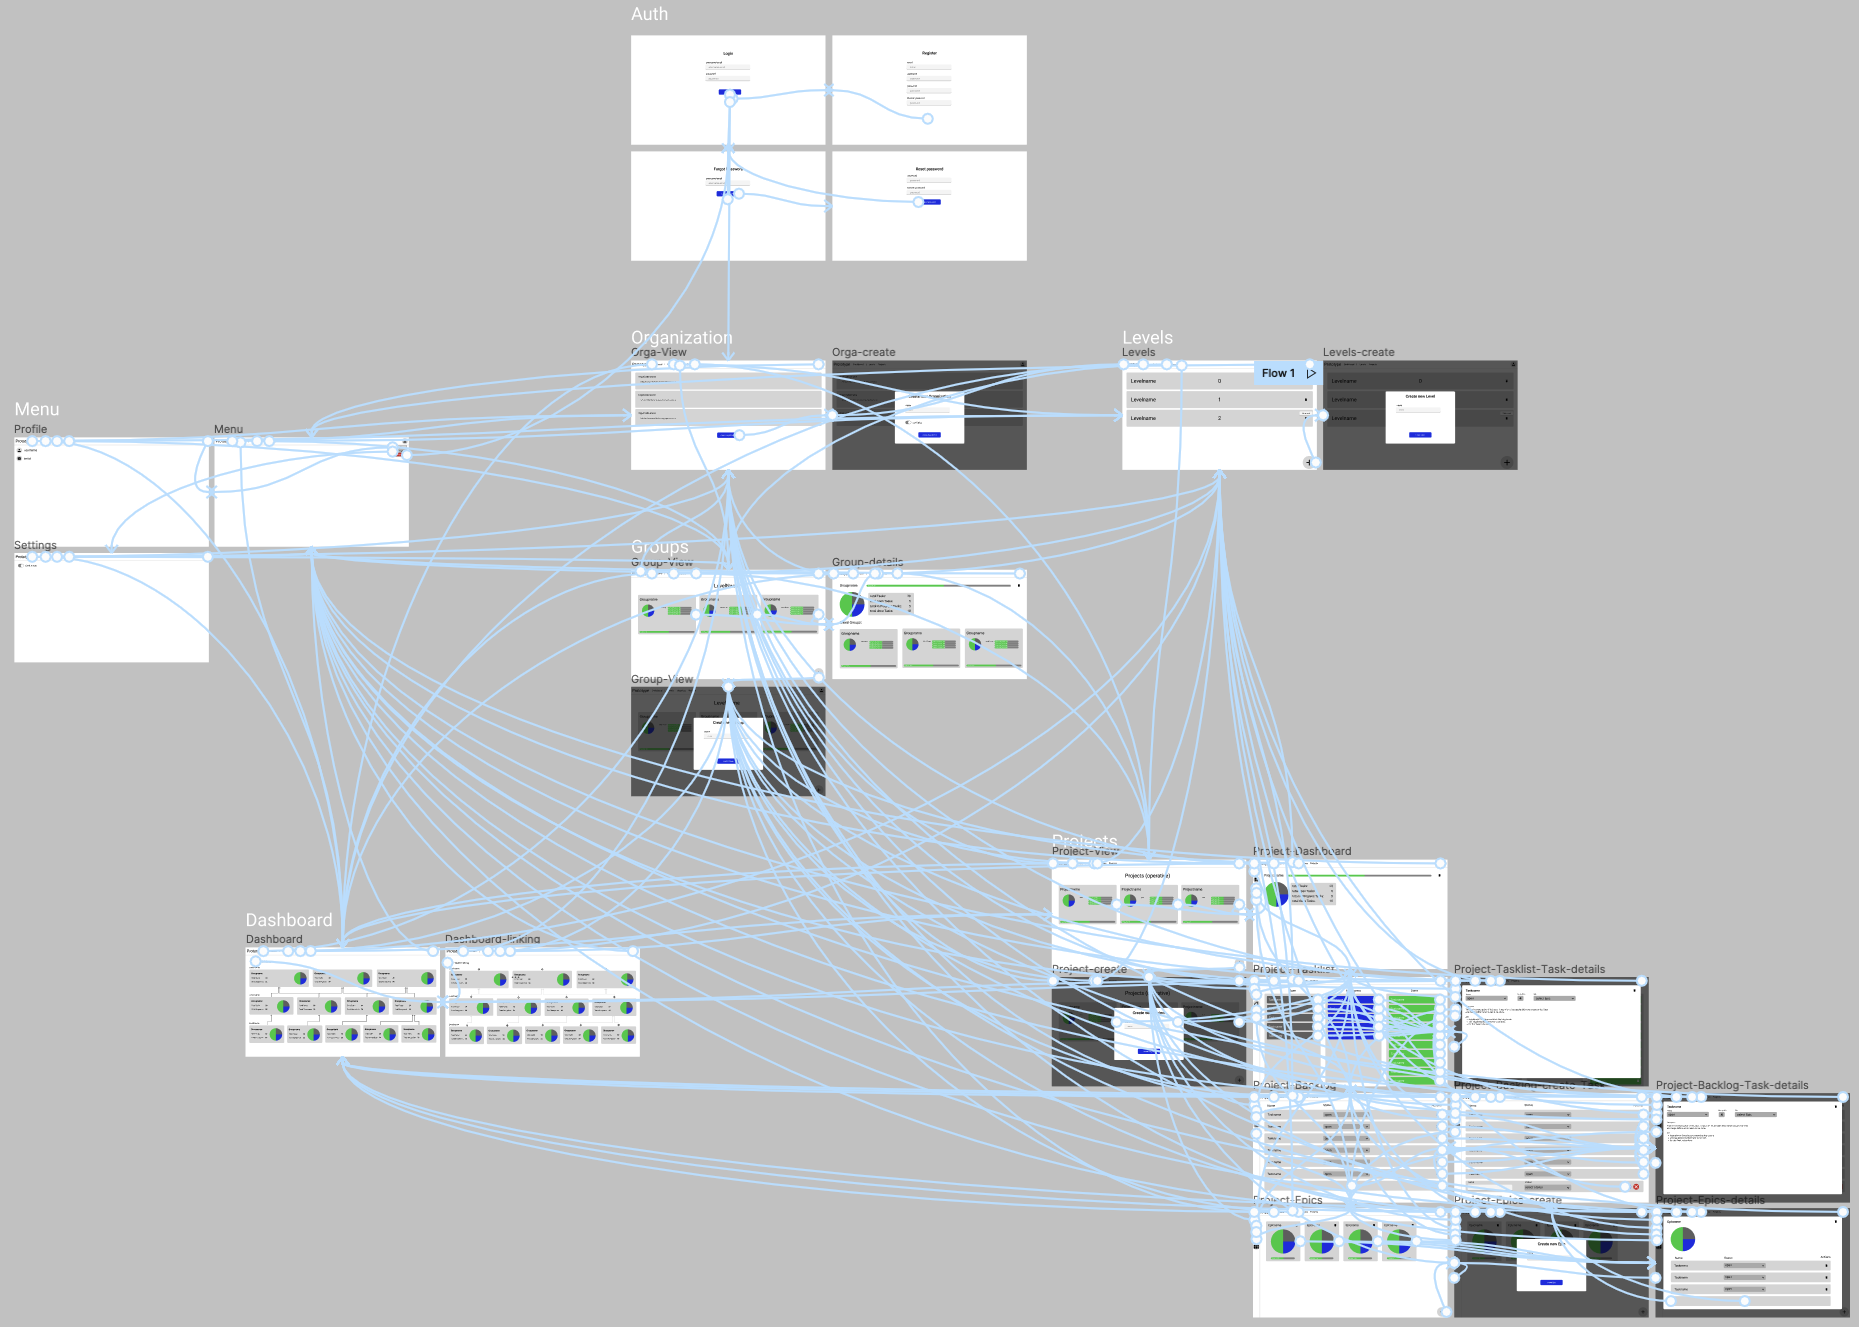
\includegraphics[width=\linewidth]{UX-Prototype}
        \captionof{figure}{UX-Prototyp für die Anwendung}
    \end{minipage}
\end{center}
\vspace{20pt}


Der Entwurf unterteilt die Anwendung in 7 verschiedene Teile:

\subsubsection{Authentifizierung}
Die Authentifizierung beinhaltet Seiten für den Login und die Registrierung. Außerdem muss der Nutzer sein Passwort zurücksetzen können, indem er einen Reset-Link für seine registrierte E-Mail-Adresse anfordert und über diesen Link ein neues Passwort vergeben kann.

\vspace{20pt}
\begin{center}
    \begin{minipage}{\linewidth}
        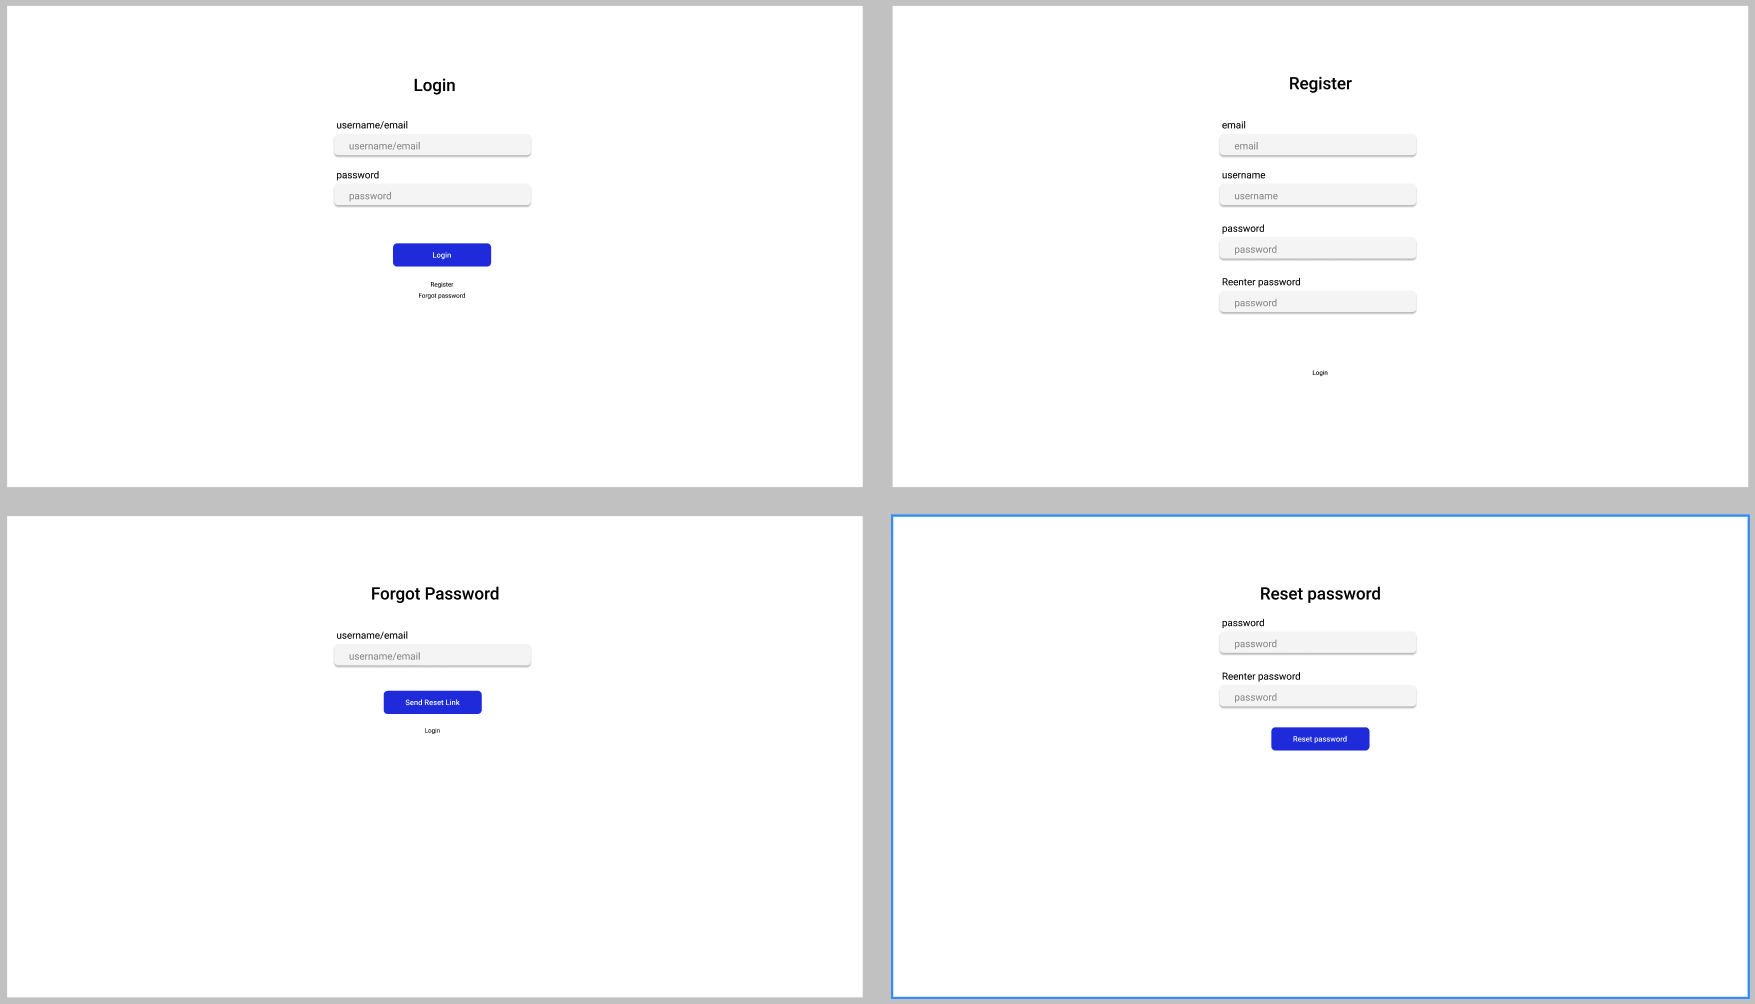
\includegraphics[width=\linewidth]{Auth}
        \captionof{figure}{UX-Prototyp für die Authentifizierung}
    \end{minipage}
\end{center}
\vspace{20pt}

\subsubsection{Menü}
Das Menü besteht aus 2 Seiten. Die Profil-Seite stellt den Nutzernamen und E-Mail-Adresse dar und ermöglicht es dem Nutzer ein JIRA-API-Token für einen JIRA-Import zu hinterlegen. Auf der Einstellungsseite kann der Nutzer zwischen Light- und Dark-Mode wechseln.

\subsubsection{Organisation}
Auf der Organisationsseite kann der Nutzer alle Organisationen sehen und neue Organisationen erstellen. Beim Erstellen einer Organisation kann der Nutzer sich entscheiden, ob er Epics verwenden möchte. Wenn die Organisation erstellt wird, wird zusätzlich ein Level für Projekte, also die unterste Ebene erstellt. Verwendet die erstellte Organisation Epics, werden 2 Ebenen standardmäßig erstellt: Project und Epic. Dies hat ebenfalls Auswirkungen auf das Dashboard, da es grundsätzlich alle Levels darstellt. Verwendet eine Organisation allerdings Epics, wird die unterste Ebene, also Epics, nicht mit dargestellt. Außerdem gibt es in den Projekten keine Möglichkeit Epics zu erstellen.

\vspace{20pt}
\begin{center}
    \begin{minipage}{\linewidth}
        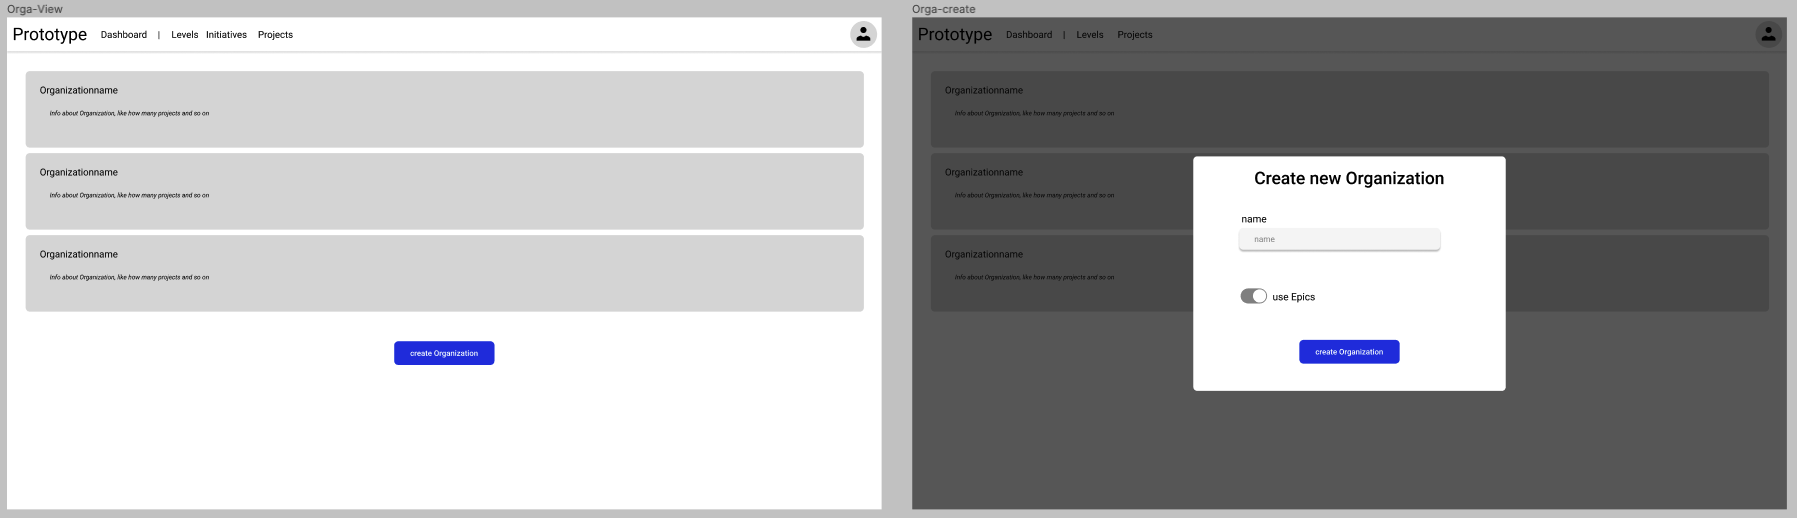
\includegraphics[width=\linewidth]{Organization}
        \captionof{figure}{UX-Prototyp für die Organisationsseite}
    \end{minipage}
\end{center}
\vspace{20pt}


\subsubsection{Dashboard}
Das Dashboard zeigt alle Planungselemente einer Organisation hierarchisch angeordnet dar und wie diese miteinander verknüpft sind. Der Nutzer kann je Element anhand einer kleinen Grafik den aktuellen Fortschritt des Elements ablesen. Außerdem hat der User die Möglichkeit den Verlinkungsmodus auszuwählen, wodurch er mit Drag-and-drop neue Verknüpfungen erstellen kann. Durch einen Klick auf das Element gelangt der Nutzer zur Detailansicht des Elements.

\vspace{20pt}
\begin{center}
    \begin{minipage}{\linewidth}
        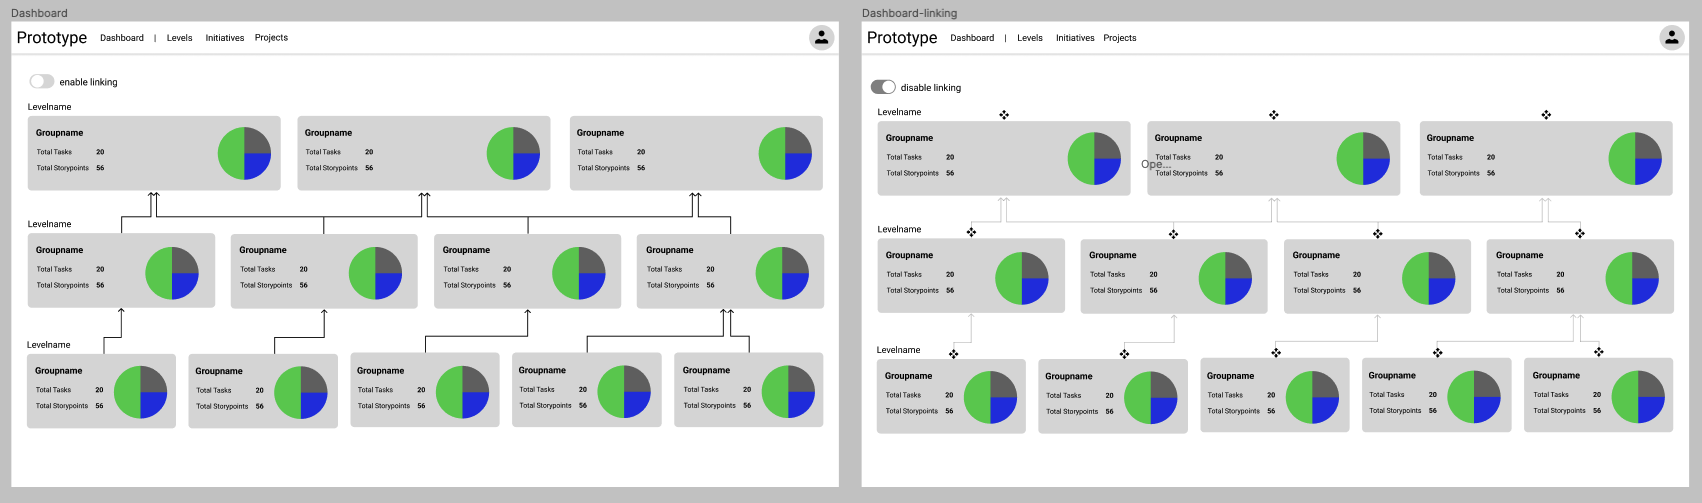
\includegraphics[width=\linewidth]{Dashboard}
        \captionof{figure}{UX-Prototyp für das Dashboard}
    \end{minipage}
\end{center}
\vspace{20pt}

\subsubsection{Levels}
Hier kann der Nutzer Ebenen(Levels) erstellen und löschen. Alle Ebenen werden hierarchisch sortiert dargestellt.

\subsubsection{Gruppen}
Je Ebene gibt es eine Gruppenansicht, die alle Elemente(Gruppen) je Level in mit einer kurzen Übersicht über den Fortschritt enthält. Der Nutzer kann neue Gruppen erstellen und auf bestehende Gruppen klicken um zu deren Detailansicht zu gelangen.
In der Gruppendetailansicht gibt es eine detaillierte Übersicht über den Fortschritt des Elements. Der Nutzer kann das Element umbenennen und löschen. Außerdem werden alle verknüpften Elemente aus der darunterliegenden Ebene dargestellt. Mit einem Klick auf eines dieser Elemente kann der Nutzer auch deren Detailansicht aufrufen.

\subsubsection{Projekt}
Die Projektübersicht ähnelt der Gruppenansicht, bietet aber zusätzlich zur einfachen Erstellung neuer Elemente auch die Möglichkeit eines Imports mit einer Excel-Datei. Außerdem kann ein Nutzer, der ein gültiges JIRA-API-Token in seinem Profil gespeichert hat, JIRA-Projekte importieren. Bei einem Import, unabhängig ob aus einer Excel-Datei oder von JIRA, wird nicht nur ein Projekt-Element erstellt, sondern ebenfalls Aufgaben innerhalb des Projekts, die aus der Excel-Datei oder JIRA ausgelesen wurden.
Durch einen Klick auf ein Element innerhalb der Übersicht gelangt der Nutzer ebenfalls in eine Detailansicht, welche sich allerdings stark von der einer gewöhnlichen Gruppe unterscheidet.

Der Nutzer kann ein Aufgaben-Board öffnen, in dem er alle Aufgaben des Projekts in drei Spalten sehen kann. Jede Spalte stellt einen der drei Fortschritts-Stati dar: \emph{open}, \emph{in progress} und \emph{done}. Der Nutzer kann mit Drag-and-drop den Status der Aufgaben ändern, indem er sie in die entsprechende Spalte bewegt. Jedes Element besitzt ein Löschsymbol, mit dem das Element, nach einer Bestätigung, gelöscht werden kann. Durch einen Klick auf ein Element öffnet sich ein Pop-up-Fenster mit der Detailansicht der Aufgabe. Diese stellt den Aufgabennamen, die Beschreibung und Storypoints sowie ggf. das zugeordnete Epic dar. Möchte der Nutzer das Epic der Aufgabe wechseln oder sie einem Epic zuordnen, kann er mit einem Drop-down-Menü aus einem der erstellen Epics auswählen. Außerdem kann der Nutzer auch hier die Aufgabe löschen.

Im Aufgaben-Backlog kann der Nutzer alle Aufgaben des Projekts als Listenansicht sehen. Er kann den Aufgabennamen ändern, den Status jeder Aufgabe mit einem Drop-down-Menü anpassen oder die Aufgabe löschen. Außerdem kann der Nutzer hier eine neue Aufgabe erstellen.

Befindet sich das Projekt in einer Organisation die Epics verwendet, gibt es ebenfalls die Epic-Übersicht. Hier werden alle Epics in dem Projekt dargestellt und ihr Fortschritt mit einer Grafik visualisiert. Der Nutzer kann neue Epics erstellen und bestehende Löschen. Klickt er auf ein Epic öffnet sich die Epic-Detailansicht in einem Pop-up-Fenster, in dem das Epic umbenannt oder gelöscht werden kann. Außerdem wird eine Liste aller Aufgaben ähnlich wie im Backlog angezeigt, die sich in dem Epic befinden. Hier kann der Nutzer zudem Aufgaben, die noch keinem Epic zugeordnet wurden, auswählen und zu diesem Epic hinzufügen. Aufgaben die sich bereits in dem Epic befinden können gelöscht oder nur aus dem Epic entfernt werden. Erstellt der Nutzer an dieser Stelle eine Aufgabe wird diese automatisch dem Epic hinzugefügt.

Das Projekt-Dashboard vereint eine Zusammenfassung des Projekt-Fortschritts mit dem Aufgaben-Board und dem Backlog.

\subsection{Datenaggregation}
Für die Fortschrittsaggregation müssen rekursiv Verknüpfungen zu Elementen der Ebene darunter zusammengefasst werden, bis die Elemente Aufgaben sind, deren Status feststeht. Hierzu beinhalten alle verknüpfbaren Elemente eine Liste mit Referenzen auf verknüpfte Elemente aus der darüber liegenden Ebene. Somit kann überprüft werden welche Elemente der darunterliegenden Ebene mit dem Element, dessen Fortschritt aggregiert werden soll, verknüpft sind. Daraus resultiert eine Liste an Elementen, bei der für jeden Eintrag der Liste genauso wie das für eigentliche Element geprüft werden kann, welche Elemente der darunter liegenden Ebene eine Referenz auf das Element haben. Dies wird so oft wiederholt, bis die verknüpften Elemente Aufgaben sind.

\vspace{20pt}
\begin{center}
    \begin{minipage}{0.8\linewidth}
        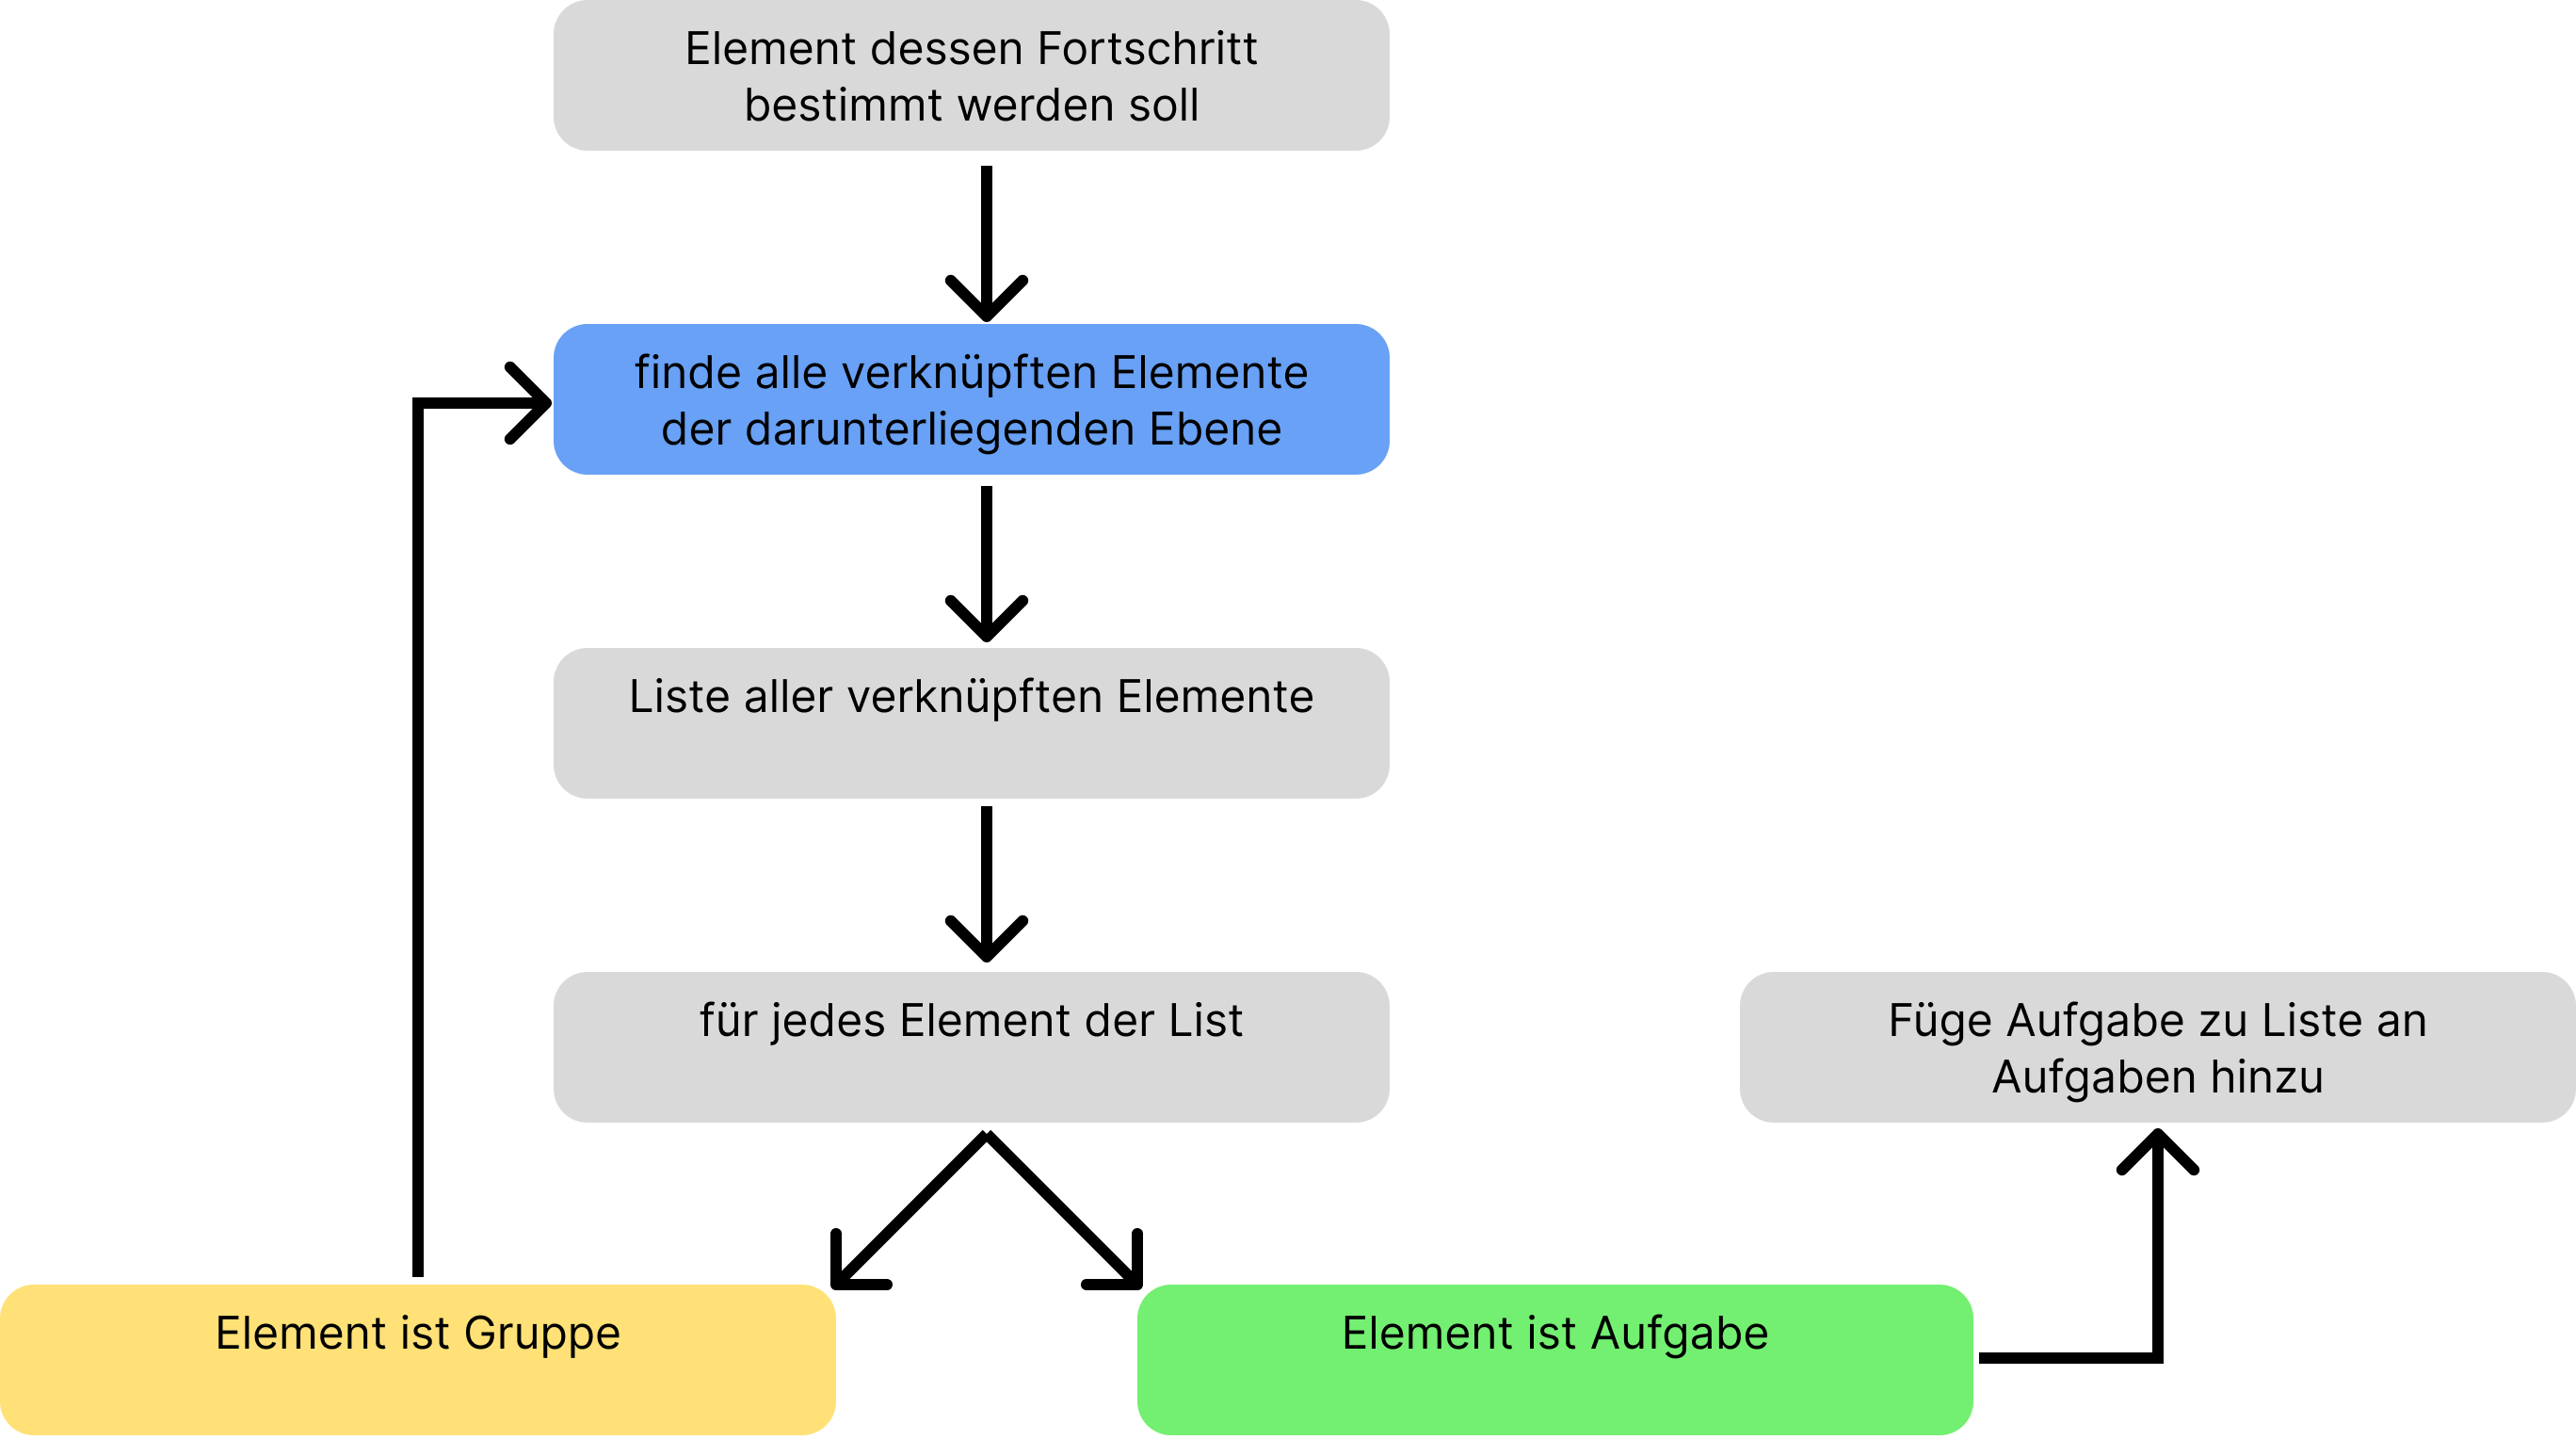
\includegraphics[width=\linewidth]{Fortschrittsaggregation}
        \captionof{figure}{Prozess für Fortschrittsaggregation}
    \end{minipage}
\end{center}
\vspace{20pt}

Die Liste an Aufgaben, die sich am Ende des Prozesses ergibt, kann anschließend nach Aufgaben in den verschiedenen Stati sortiert werden. Aus diesen Listen können nun 3 verschiedene Fortschrittsvarianten berechnet werden. Die Anzahl an fertigen Aufgaben geteilt durch die Gesamtmenge an Aufgaben ergibt einen absoluten Fortschritt. Für einen relativen Fortschritt kann die Summe der Storypoints oder des Values aller fertigen Aufgaben durch die Gesamtmenge an Storypoints oder des Values aller Aufgaben geteilt werden, um den relativen Fortschritt zu bestimmen.
